\chapter{Implementazione e manuale utente}

\begin{preamble}
{\em Il capitolo seguente è uno dei più importanti in quanto mostrerà, nella prima parte, la modalità di creazione ed importazione di un nuovo oggetto tridimensionale all'interno dell'applicazione Unity. \newline \indent Successivamente, verranno mostrate le implementazioni, in codice C\#, delle classi descritte nei Class Diagram del capitolo precedente. Inoltre, si descriveranno nel dettaglio le modalità di creazione delle animazioni impiegate del menù principale e nella scena dedicata alla selezione dell'annata del prodotto vitivinicolo. \newline \indent L'ultima sezione è dedicata al manuale utente che fornirà un guida all'utilizzo dell'applicazione da parte dell'utente.}
\end{preamble}

\section{Creazione ed importazione di un modello tridimensionale di un prodotto}
\subsection{Creazione del modello tridimensionale dell'oggetto tramite smartphone}

In questa sezione si descriverà il processo di creazione ed importazione di un modello tridimensionale di un prodotto vitivinicolo per permettere poi a Vuforia Engine di effettuarne il riconoscimento tramite l'applicazione Android sviluppata in Unity.

Come già accennato nei capitoli precedenti, il primo passo consiste nella creazione di un primo modello tridimensionale tramite l'applicazione mobile PolyCam. Dopo aver creato un account tramite l'apposito form presente nell'applicazione, per la creazione del modello tridimensionale impiegato nel progetto si è scelta la modalità \textit{Photo Mode}. essa consiste nell'acquisizione tramite fotocamera di un serie di fotografie all'oggetto di cui vogliamo creare un modello tridimensionale.

Per ottenere un modello di alta qualità, PolyCam consiglia di inserire l'oggetto all'interno di un piccolo set fotografico composto in questo modo: bisogna eliminare ogni fonte di "rumore" o "disturbo" presente nello sfondo del set fotografico. In altre parole, bisogna posizionare dietro l'oggetto un telo o anche un cartoncino scuro che impedisca ad altri oggetti di essere coinvolti nella creazione del modello tridimensionale. Per il progetto, è stata utilizzata una scatola di cartone posta dietro alla bottiglia di vino della cantina Strappelli (Figura \ref{}).

\begin{figure}[h]
	\centering
	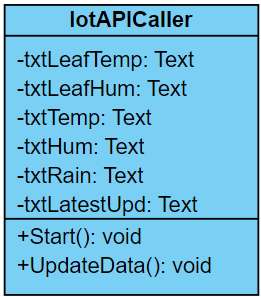
\includegraphics [width=.30\columnwidth, angle=0]
            {ClassDiagramIotAPICaller}
	\caption{Class Diagram della classe IotAPICaller}
	\label{5fig:classDiagramIotAPICaller}
\end{figure}

In secondo luogo, le foto devono essere scattate in modo tale da avere una panoramica a 360$^\circ$ della bottiglia. Per ottenere ciò, la bottiglia è stata posta sopra una piattaforma girevole per consentire la rotazione dell'oggetto mentre si acquisivano le immagini in sequenza dello stesso.

Una volta ottenute le immagini dell'oggetto, esse vengono inviate al server di PolyCam che in poco tempo fornisce un modello tridimensionale dell'oggetto desiderato in formato glTF.

\subsection{Raffinamento del modello tridimensionale con Blender}

Il modello tridimensionale fornito da PolyCam molto probabilmente presenta delle imperfezioni dovute al rumore che è presente nelle varie immagini acquisite. Ad esempio, nel caso della bottiglia di vino, è stato necessario rimuovere delle imperfezioni presenti sopra e sotto l'oggetto in quanto rappresentavano porzioni dello sfondo che PolyCam ha erroneamente incluso all'interno del modello tridimensionale.
Di seguito sono riportati il modello prima (Figura \ref{}) e dopo (\ref{}) le correzioni effettuate in Blender. 

\subsection{Creazione ed importazione di un modello in Vuforia Engine}

Una volta corretto il modello, è possibile esportarlo nel formato glTF richiesto da Vuforia. Successivamente è necessario creare un account e quindi una licenza gratuita sul portale sviluppatori di Vuforia. La licenza ottenuta dovrà essere poi riportata all'interno del software \textit{Vuforia Model Target Generator} per permetterne il regolare utilizzo.

Una volta aver aperto il programma ed aver poi inserito la licenza di Vuforia, è possibile importare il modello glTF creato in precedenza all'interno di Vuforia Model Target Generator. Quest'ultimo, rielaborerà il modello nel formato glTF in modo tale da essere poi importato in Unity.

In quest'ultimo, è possibile importare Vuforia Engine tramite il package manager. Una volta importato, nella scena Unity dedicata al riconoscimento delle bottiglie (Figura \ref{})
è inserito un oggetto chiamato \textit{Model Target} che ingloba al suo interno gli strumenti del motore grafico Vuforia per attuare il riconoscimento del prodotto vitivinicolo. 
All'interno di questo oggetto Unity, è presente uno script C\# chiamato \textit{ObjectTrackingHandler} che contiene una classe omonima e un metodo in particolare chiamato \textit{OnTrackingFound}. Quest'ultimo permette di stabilire le operazioni da effettuare nel momento in cui il riconoscimento della bottiglia è avvenuto con successo. Ciò che viene fatto nell'applicazione Android è quello di salvare all'interno di una variabile chiamata \textit{\_trackedObjectName} il nome dell'oggetto riconosciuto e successivamente caricare la scena successiva dedicata alla selezione dell'annata di riferimento del vino.


\section{Implementazione delle classi principali}

Nel capitolo precedente, sono stati forniti i Class Diagram delle classi più importanti che permettono di implementare le funzionalità principali dell'applicazione Android. In questa sezione, si mostrerà il codice per ognuna delle classi impiegate.

\subsection{Implementazione della classe IotAPICaller}



\subsection{Implementazione della classe OpenWeatherAPICaller}



\subsection{Implementazione della classe ScriptManager}



\subsection{Implementazione della classe MongoDBConnector}



\section{Implementazione delle animazioni in Unity}
\subsection{Menù principale}
\subsection{Selezione dell'annata}

\section{Manuale utente}
\subsection{Premessa}

Normalmente, un'applicazione Android è presente nel Google Play Store da cui è possibile scaricarla ed installarla in pochi minuti. Purtroppo quest'applicazione essendo un prototipo, non è ancora presente in questa piattaforma. Questa è la ragione per cui necessita di alcuni passaggi aggiuntivi per essere installata correttamente. In futuro, se il progetto prenderà piede, l'applicazione sarà caricata all'interno del Google Play Store per essere aumentare l'accessibilità del prodotto.

\subsection{Effettuare il riconoscimento di un prodotto}
\subsection{Utilizzo delle sezioni principali}